\chapter{Implementación hardware}

Para implementar el algoritmo en hardware dividimos en modulos el algoritmo de filtrado, el algoritmo
de deteccion de picos y el algoritmo de deteccion de arritmias, estos los unificamos en un super modulo 
y probamos la simulacion con un testbench.

Como los valores de las señales estan en punto flotante para operar con ellos es necesario utilizar modulos
hardware que permitan hacer dichas operaciones, en este proyecto utilizaremos modulos de resta, division y 
comparacion de numeros en punto flotante.

Por tanto en esta imagen quedan representados todos los modulos.

(IMAGEN DE MODULOS Y QUIEN LOS IMPLEMENTA)

\section{Modulo de filtrado}

Este modulo utiliza una ROM con los coeficientes, una RAM con las muestras y un modulo de multiplicacion
de numeros en punto flotante.

Este modulo se compone de una maquina de estados que va multiplicando cada elemento de la RAM muestras 
con los elementos de la ROM coeficientes con el modulo de multiplicacion de punto flotante.

\subsection{Señales de entrada y salida}

Las señales de entrada son:

\begin{itemize}
\item clk y reset
\item input\_signal\_data: señal que recibe las muestras de la señal original 
\item input\_valid e input\_ready: son flags que sirven para sincronizar el modulo con la llegada de muestras. 
\end{itemize}

Las señales de salida son:

\begin{itemize}
    \item output\_filter\_data: saca los valores de la señal filtrada
    \item output\_filter\_index: saca los indices de cada valor de la señal filtrada
    \item output\_valid y output\_ready: se encargan de sincronizar el modulo del filtrado 
    con el modulo de deteccion de picos
\end{itemize}

\lstset{language=VHDL, breaklines=true, basicstyle=\footnotesize}
\begin{lstlisting}[frame=single]
    entity filter is
    port (
        -- Seniales de reloj y de reset
        clk                 : in  std_logic;
        reset               : in  std_logic; 
        
        -- bus AXI Stream de entrada
        input_signal_data   : in  std_logic_vector(31 downto 0);
        input_valid         : in  std_logic;
        input_ready         : out std_logic;
        
        -- bus AXI Stream de salida
        output_filter_data  : out std_logic_vector(31 downto 0);
        output_filter_index : out std_logic_vector(31 downto 0);
        output_valid        : out std_logic;
        output_ready        : in  std_logic   
   );
end filter;
\end{lstlisting}

\subsection{Maquina de estados}

Se realiza el proceso de sincronizacion de los estados, donde las señales siguientes pasan a las señales actuales.

\lstset{language=VHDL, breaklines=true, basicstyle=\footnotesize}
\begin{lstlisting}[frame=single]
    sync: process(clk)
    begin
        if ( rising_edge(clk) ) then
            if ( reset = '1' ) then
                state <= estado_espera;
                cont_muestras <= (others=>'0');
                cont_coeficientes <= (others=>'0');
                cont_indice <= (others=>'0');
                acumulado <= (others=>'0');
            else
                state <= next_state;
                cont_muestras <= next_cont_muestras;
                cont_coeficientes <= next_cont_coeficientes;
                cont_indice <= next_cont_indice;
                acumulado <= next_acumulado;                
            end if;
        end if;
    end process sync;
\end{lstlisting}

Se realiza el proceso de actualizacion de las señales donde se le asignan nuevos valores para el siguiente ciclo de reloj.

\begin{itemize}
    \item Estado de espera: En el estado de espera se activa la señal de ready y se espera a que se envie un valor de la
    señal sin filtrar, se borra el valor de la solucion de la multiplicacion anterior en caso de haberla, se activan las
    señales de escritura de la RAM y se establece el indice donde se va a escribir la muestra.
    \item Estado lectura: Se activa la lectura de los coeficientes y de las muestras.
    \item Estado para ordenar el cálculo: en este estado se activa el flag del modulo de multiplicacion.
    \item Estado de espera del calculo: se espera a que termine el modulo de multiplicacion esperando la señal de ready\_muladd
    y se almacena el resultado, tambien se actualiza el contador de los coeficientes, de las muestras y dependiendo de si el 
    indice de coeficientes es menor que 98 se va al estado de lectura o el estado de enviar un nuevo dato al siguiente modulo.
    \item Estado de envio de nuevo dato: este estado sincroniza el siguientemodulo, activa el bit de valid a 1 y espera el bit
    de ready del siguiente modulo para poder enviar el dato.
\end{itemize}

\lstset{language=VHDL, breaklines=true, basicstyle=\footnotesize}
\begin{lstlisting}[frame=single]
    cmb: process(state, cont_coeficientes, cont_muestras, cont_indice, acumulado, input_valid, ready_muladd, result_muladd, output_ready)
    begin
        -- Registros de estado y de seniales
        next_state <= state;
        next_cont_coeficientes <= cont_coeficientes;
        next_cont_muestras <= cont_muestras;
        next_acumulado <= acumulado;
        next_cont_indice <= cont_indice;
        
        -- Seniales de control de los buses
        input_ready <= '0';
        output_valid <= '0';
        
        -- Seniales de control para la ruta de datos
        ROM_coeficientes_ena <= '0';
        RAM_muestras_ena <= '0';
        RAM_muestras_wea <= "0";
        enable_muladd <= '0';
  
        case state is 
            
            when estado_espera =>
                input_ready <= '1';
                if ( input_valid = '1' ) then
                    next_acumulado <= (others=>'0');
                    -- Almacenamos el valor de entrada
                    RAM_muestras_ena <= '1';
                    RAM_muestras_wea <= "1";
                    if ( to_integer(unsigned(cont_muestras)) < 98 ) then
                        next_cont_muestras <= std_logic_vector(unsigned(cont_muestras) + 1);                        
                    else
                        next_cont_muestras <= (others=>'0');
                    end if;
                    next_state <= estado_lectura;
                end if;
                 
            when estado_lectura => 
                -- Hacemos la lectura de ambas memorias  
                ROM_coeficientes_ena <= '1';
                RAM_muestras_ena <= '1';
                next_state <= estado_ordenar_calculo;
                
            when estado_ordenar_calculo =>
                enable_muladd <= '1';
                next_state <= estado_espera_calculo;
                            
            when estado_espera_calculo =>
                if ( ready_muladd = '1' ) then
                    next_acumulado <= result_muladd;
                    
                    if ( to_integer(unsigned(cont_muestras)) < 98 ) then
                        next_cont_muestras <= std_logic_vector(unsigned(cont_muestras) + 1);                        
                    else
                        next_cont_muestras <= (others=>'0');
                    end if;
                    
                    if ( to_integer(unsigned(cont_coeficientes)) < 98 ) then
                        next_cont_coeficientes <= std_logic_vector(unsigned(cont_coeficientes) + 1);                        
                    else
                        next_cont_coeficientes <= (others=>'0');
                    end if;                    
                    
                    if ( to_integer(unsigned(cont_coeficientes)) < 98 ) then
                        next_state <= estado_lectura;
                    else
                        next_state <= estado_enviar_nuevo_dato;
                    end if;
                    
                end if;
            
            when estado_enviar_nuevo_dato =>      
                output_valid <= '1';
                if ( output_ready = '1' ) then
                    next_cont_indice <= std_logic_vector(unsigned(cont_indice) + 1);
                    next_state <= estado_espera;
                end if;

        end case;
    end process cmb;
\end{lstlisting}

El envio de datos al output se realiza de forma asincrona
\lstset{language=VHDL, breaklines=true, basicstyle=\footnotesize}
\begin{lstlisting}[frame=single]
    output_filter_data <= acumulado;
    output_filter_index <= cont_indice;
\end{lstlisting}

\subsection{Modulos utilizados}
Se utilizo una ROM para almacenar los coeficientes y poder leerlos

\lstset{language=VHDL, breaklines=true, basicstyle=\footnotesize}
\begin{lstlisting}[frame=single]
    -- ROM que contiene los coeficientes 
    ROM_coeficientes_i : entity work.ROM_coeficientes port map (
        clka      => clk,
        ena       => ROM_coeficientes_ena,
        addra     => ROM_coeficientes_addra,
        douta     => ROM_coeficientes_douta
    );
    
    ROM_coeficientes_addra <= cont_coeficientes;
\end{lstlisting}

Se usa una RAM para poder leer y escribir en las muestras de la señal original.

\lstset{language=VHDL, breaklines=true, basicstyle=\footnotesize}
\begin{lstlisting}[frame=single]
    -- ROM que contiene las muestras 
    RAM_muestras_i : entity work.RAM_muestras port map (
        clka      => clk,
        ena       => RAM_muestras_ena,
        wea       => RAM_muestras_wea,
        addra     => RAM_muestras_addra,
        dina      => RAM_muestras_dina,
        douta     => RAM_muestras_douta
    );    
    
    RAM_muestras_addra <= cont_muestras;
    RAM_muestras_dina <= input_signal_data;
\end{lstlisting}

Se usa un modulo de multiplicacion para poder multiplicar los valores de las muestras con los valores de los coeficientes.

\lstset{language=VHDL, breaklines=true, basicstyle=\footnotesize}
\begin{lstlisting}[frame=single] 
    -- Multiplicacion y suma 
    mul_add_i : entity work.muladdpf port map (
        aclk                    => clk,
        s_axis_a_tvalid         => enable_muladd,
        s_axis_a_tdata          => RAM_muestras_douta,
        s_axis_b_tvalid         => enable_muladd,
        s_axis_b_tdata          => ROM_coeficientes_douta,
        s_axis_c_tvalid         => enable_muladd,
        s_axis_c_tdata          => acumulado,                
        m_axis_result_tvalid    => ready_muladd,
        m_axis_result_tdata     => result_muladd
    );
\end{lstlisting}

\section{Modulo de deteccion de picos}

Este modulo se encarga de detectar los picos de la señal filtrada. 
\subsection{Señales de entrada y salida}
    \begin{itemize}
    \item clk y reset
    \item input\_signal\_data: señal que recibe las muestras de la señal filtrada 
    \item input\_signal\_index: señal que recibe lso indices de las muestras de la señal filtrada 
    \item input\_valid e input\_ready: son flags que sirven para sincronizar el modulo con la llegada de muestras. 
    \end{itemize}
    
    Las señales de salida son:
    
    \begin{itemize}
        \item output\_peak\_index: saca los indices de los picos detectados
        \item output\_valid y output\_ready: Se encargan de sincronizar el modulo de deteccion de picos 
        con el modulo de deteccion de arritmias.
    \end{itemize}
    
\lstset{language=VHDL, breaklines=true, basicstyle=\footnotesize}
\begin{lstlisting}[frame=single] 
port (
    -- Seniales de reloj y de reset
    clk                 : in  std_logic;
    reset               : in  std_logic; 
    
    -- bus AXI Stream de entrada
    input_signal_data   : in  std_logic_vector(31 downto 0);
    input_signal_index  : in  std_logic_vector(31 downto 0); -- vamos a dejarlo en 32 (aunque no sean necesarios tantos bits) para sean todos los buses iguales
    input_valid         : in  std_logic;
    input_ready         : out std_logic;
    
    -- bus AXI Stream de salida
    output_peak_index   : out std_logic_vector(31 downto 0); -- vamos a dejarlo en 32 (aunque no sean necesarios tantos bits) para sean todos los buses iguales
    output_valid        : out std_logic;
    output_ready        : in  std_logic   
);
\end{lstlisting}
\subsection{Maquina de estados}
Se realiza el proceso de sincronizacion de los estados, donde las señales siguientes pasan a las señales actuales.

\lstset{language=VHDL, breaklines=true, basicstyle=\footnotesize}
\begin{lstlisting}[frame=single]
    sync: process(clk)
    begin
        if ( rising_edge(clk) ) then
            if ( reset = '1' ) then
                state <= estado_espera;
                signal_data <= (others=>'0');
                signal_index <= (others=>'0');
                last_peak <= (others=>'0');
                last_index <= (others=>'0');
                cutoff <= (others=>'0');
            else
                state <= next_state;
                signal_data <= next_signal_data;
                signal_index <= next_signal_index;
                last_peak <= next_last_peak;
                last_index <= next_last_index; 
                cutoff <= next_cutoff;
            end if;
        end if;
    end process sync;
\end{lstlisting}

Se realiza el proceso de actualizacion de las señales donde se le asignan nuevos valores para el siguiente ciclo de reloj.

\begin{itemize}
    \item Estado de espera: En el estado de espera se activa la señal de ready y se espera a que se envie un valor de la
    señal sin filtrar, se borra el valor de la solucion de la multiplicacion anterior en caso de haberla, se activan las
    señales de escritura de la RAM y se establece el indice donde se va a escribir la muestra.
    \item Estado de comprobar indice: si no hay pico, o lo que es lo mismo que la señal de last\_peak este a 0 este se asigna
     a la señal y ademas se registra el indice, despues pasa al estado de actualizar el cutoff activando por tanto la señal de 
     division para que empiecen los modulos de division y resta de valores en punto flotante a calcular el valor. Si por otro
     lado si que hay pico, se ordena hacer la comparacion signal\_data > last\_peak pasando las señales correspondientes al modulo de comparacion en 
     punto flotante. Ademas se anticipa y se hace la comparacion last\_peak > cutoff para en dado caso de que no se cumpla la 
     condicion anterior ya esta la comparacion hecha y se pude pasar directamente al estado siguiente. Tambien activamos las señales
     del modulo de comparacion correspondiente. El siguiente estado es el estado de espera a la condicion en la que la señal es mayor 
     que el pico maximo.
    \item Estado de actualizar cutoff: este estado espera a la señal ready del modulo de la resta ya que es la ultima operacion que se realiza para 
    calcular el cutoff. Primero se ejecuta el modulo de la division para calcular cutoff/192 y luego la resta cutoff - cutoff/192. cuando la señal
    ready\_sub sea '1' se actualiza el cutoff y pasa al estado de espera terminando la iteracion. 
    \item Estado de espera a la condicion en la que la señal es mayor que el pico maximo: cuando las señales ready de los comparadores esten a '1' 
    se podra ejecutar las funcionalidades del estado. este tiene 3 condiciones:
    \begin{itemize}
        \item si se ha encontrado un valor mas alto que last\_index, este pico pasa a ser el nuevo last\_peak y el nuevo cutoff, el index tambien se actualiza. 
        \item la señal result\_signal\_index\_sub\_last\_index\_gt\_or\_eq\_samples\_around\_peak se calcula de forma asincrona, por lo que si esa condicion que
         indica que han pasado 72 muestras sin encontrar un valor mas alto que last\_peak y ademas last\_peak es mayor que el cutoff, se pasa directamente al estado
         de envio de nuevo pico para enviar el pico QRS.
        \item Sino simplemente se ordena la actualizacion del cutoff activando el enable del modulo de la division y pasando al estado correspondiente.
    \end{itemize}
    \item Estado de envio de nuevo pico: se activa la señal de valid a 1 y espera a que el modulo de deteccion de arritmias mande la señal de ready para resetear 
    las señales de last peak y last index a '0' ademas se actualiza el cutoff.
\end{itemize}
\lstset{language=VHDL, breaklines=true, basicstyle=\footnotesize}
\begin{lstlisting}[frame=single]
    cmb: process(state, signal_data, signal_index, last_peak, last_index, cutoff, input_valid, input_signal_data, input_signal_index, ready_signal_data_gt_cutoff, result_signal_data_gt_cutoff, ready_sub, result_sub, ready_signal_data_gt_last_peak, result_signal_data_gt_last_peak, result_signal_index_sub_last_index_gt_or_eq_samples_around_peak, result_last_peak_gt_cutoff, output_ready,samples_around_peak)
    begin
        -- Registros de estado y de seniales
        next_state <= state;
        next_signal_data <= signal_data;
        next_signal_index <= signal_index;
        next_last_peak <= last_peak;
        next_last_index <= last_index;
        next_cutoff <= cutoff;
        
        -- Seniales de control de los buses
        input_ready <= '0';
        output_valid <= '0';
        
        -- Seniales de control para la ruta de datos
        enable_signal_data_gt_cutoff <= '0';
        enable_div <= '0';
        enable_signal_data_gt_last_peak <= '0';
        enable_last_peak_gt_cutoff <= '0';
    
        case state is 
        
            -- Esperamos a que llegue una nueva muestra
            when estado_espera =>
                -- El modulo esta listo para recibir nuevos datos
                input_ready <= '1';
                if ( input_valid = '1' ) then
                    -- Almaceno los valores de entrada
                    next_signal_data <= input_signal_data;
                    next_signal_index <= input_signal_index;
                    next_state <= estado_comprueba_indice;
                 end if;
                 
            when estado_comprueba_indice =>
                if ( to_integer(unsigned(signal_index)) < unsigned(samples_around_peak)) then  -- Las primeras 300 muestras las utilizamos para fijar un cutoff inicial
                    next_state <= estado_espera;
                else
                    if ( last_peak = x"00000000" ) then
                        next_last_peak <= signal_data;
                        next_last_index <= signal_index;
                        -- ordenar la actualizacion del cutoff (division)
                        enable_div <= '1';
                        next_state <= estado_actualizar_cutoff;
                    else
                        -- Ordenamos hacer la comparacion 'signal[i] > last_peak'
                        enable_signal_data_gt_last_peak <= '1';
                        enable_signal_data_gt_cutoff <= '1';
                        
                        enable_last_peak_gt_cutoff <= '1';
                        next_state <= estado_espera_condicion_signal_data_gt_last_peak;
                    end if;
                end if;
                
            when estado_actualizar_cutoff =>
                -- Ha terminado la resta
                if ( ready_sub = '1' ) then
                    next_cutoff <= result_sub;
                    next_state <= estado_espera;
                end if;                
                
             when estado_espera_condicion_signal_data_gt_last_peak =>
                if ( ready_signal_data_gt_last_peak = '1' and ready_signal_data_gt_cutoff = '1') then
                    if ( result_signal_data_gt_last_peak(0) = '1' and result_signal_data_gt_cutoff(0) = '1') then
                        next_last_peak <= signal_data;
                        next_last_index <= signal_index;
                        next_cutoff <= signal_data;
                        next_state <= estado_espera;
                    elsif ( result_signal_index_sub_last_index_gt_or_eq_samples_around_peak ='1' and result_last_peak_gt_cutoff(0) = '1' ) then                     
                        -- Hemos encontrado un nuevo pico
                        next_state <= estado_envio_nuevo_pico;
                    else
                        -- ordenar la actualizacion del cutoff (division)
                        enable_div <= '1';
                        next_state <= estado_actualizar_cutoff;
                    end if;
                end if;
                
              when estado_envio_nuevo_pico =>
                    -- output_peak_index <= last_index;
                    output_valid <= '1';
                    if ( output_ready = '1' ) then
                        next_last_peak <= (others => '0');
                        next_last_index <= (others => '0');
                        enable_div <= '1';
                        next_state <= estado_actualizar_cutoff;
                    end if;
                
        end case;
    end process cmb;
\end{lstlisting}

De manera asincrona se pasa como output el last index pero el modulo de deteccion de arritmias se activa cuando input\_valid
se activa usando asi el last index correspondiente 
\lstset{language=VHDL, breaklines=true, basicstyle=\footnotesize}
\begin{lstlisting}[frame=single]
    output_peak_index <= last_index;
\end{lstlisting}

\subsection{Módulos utilizados}

Se usa un modulo de comparador para 2 comparaciones, y uno de division y otro de resta para calcular el cutoff
(TODO IMAGEN DE LOS MODULOS)
\lstset{language=VHDL, breaklines=true, basicstyle=\footnotesize}
\begin{lstlisting}[frame=single]
-- Comparador 'signal[i] > cutoff' 
signal_data_gt_cutoff : entity work.gtFP port map (
    aclk                  => clk,
    s_axis_a_tvalid       => enable_signal_data_gt_cutoff,
    s_axis_a_tdata        => signal_data,
    s_axis_b_tvalid       => enable_signal_data_gt_cutoff,
    s_axis_b_tdata        => cutoff,
    m_axis_result_tvalid  => ready_signal_data_gt_cutoff,
    m_axis_result_tdata   => result_signal_data_gt_cutoff
);

-- Divisor 'cutoff / 192'
divisor : entity work.divFP port map (
    aclk                  => clk,
    s_axis_a_tvalid       => enable_div,
    s_axis_a_tdata        => cutoff,
    s_axis_b_tvalid       => enable_div,
    s_axis_b_tdata        => x"43400000",                    -- 192 en decimal
    m_axis_result_tvalid  => ready_div,
    m_axis_result_tdata   => result_div
);

-- Restador 'cutoff - cutoff/192'
enable_sub <= ready_div;
restador : entity work.subfp port map(
    aclk                  => clk,
    s_axis_a_tvalid       => enable_sub,
    s_axis_a_tdata        => cutoff,
    s_axis_b_tvalid       => enable_sub,
    s_axis_b_tdata        => result_div,
    m_axis_result_tvalid  => ready_sub,
    m_axis_result_tdata   => result_sub
);

-- Comparacion 'signal[i] > last_peak'
signal_data_gt_last_peak: entity work.gtFP port map(
    aclk                  => clk,
    s_axis_a_tvalid       => enable_signal_data_gt_last_peak,
    s_axis_a_tdata        => signal_data,
    s_axis_b_tvalid       => enable_signal_data_gt_last_peak,
    s_axis_b_tdata        => last_peak,
    m_axis_result_tvalid  => ready_signal_data_gt_last_peak,
    m_axis_result_tdata   => result_signal_data_gt_last_peak
);

-- Comparacion 'last_peak > cutoff'
last_peak_gt_cutoff: entity work.gtFP port map(
    aclk                  => clk,
    s_axis_a_tvalid       => enable_last_peak_gt_cutoff,
    s_axis_a_tdata        => last_peak,
    s_axis_b_tvalid       => enable_last_peak_gt_cutoff,
    s_axis_b_tdata        => cutoff,
    m_axis_result_tvalid  => ready_last_peak_gt_cutoff,
    m_axis_result_tdata   => result_last_peak_gt_cutoff
);
\end{lstlisting}
\section{Modulo de deteccion de arritmias}

El modulo de deteccion de arritmias se encarga de detectar si la distancia entre 2 picos QRS es considerada una arritmia o no,
 
\subsection{Señales de entrada y salida}
las señales de entrada de este modulo son:

\begin{itemize}
    \item clk y reset
    \item input\_peak\_index: señal que recibe las muestras de los picos QRS.
    \item input\_valid e input\_ready: son flags que sirven para sincronizar este modulo con el modulo de deteccion de picos. 
\end{itemize}
    
Las señales de salida son:

\begin{itemize}
    \item output\_arrythmia\_detected: flag que saca 0 si el ritmo es normal y 1 si se ha detectado una arritmia.
    \item output\_arrythmia\_index: valor que indica en que sample se ha producido la arritmia.
    \item output\_valid y output\_ready: para la sincronizacion con el modulo output.
\end{itemize}

\lstset{language=VHDL, breaklines=true, basicstyle=\footnotesize}
\begin{lstlisting}[frame=single]
    Port (
        clk: in std_logic;
        rst: in std_logic;
        
        input_peak_index: in std_logic_vector(31 downto 0); --por coherencia con el modulo anterior lo dejamos asi
        input_valid: in std_logic;
        input_ready: out std_logic;
        
        output_arrythmia_detected: out std_logic; -- ya que saca 0 si es ritmo normal y 1 si es arritmia
        output_arrythmia_index: out std_logic_vector(31 downto 0);
        output_valid: out std_logic;
        output_ready: in std_logic
       );
\end{lstlisting}

\subsection{Maquina de estados}
Se realiza el proceso de sincronizacion de los estados, donde las señales siguientes pasan a las señales actuales.

\lstset{language=VHDL, breaklines=true, basicstyle=\footnotesize}
\begin{lstlisting}[frame=single]
sync: process(clk,rst)
begin
    if rising_edge(clk) then
        if(rst = '1') then
            state <= estado_espera;
            peak_index <= (others=>'0');
            last_peak_index <= (others=>'0');
            act_distance <= (others=>'0');
            last_distance <= (others=>'0');
            pos_buffer0 <= (others=>'0');
            pos_buffer1 <= (others=>'0');
            pos_buffer2 <= (others=>'0');
            pos_buffer3 <= (others=>'0');
            TNRange <= '0';
            counter_arrythmias <= (others=>'0');
            counter <= (others=>'0');
            --para que no de arritmia al principio inicializo el gap a 1
            gap <= (others => '0');
            distance_for_calc <= (others => '0');
            --percentage <= '0';
        else
            state <= next_state;
            peak_index <= next_peak_index;
            last_peak_index <= next_last_peak_index;
            act_distance <= next_act_distance;
            last_distance <= next_last_distance;
            pos_buffer0 <= next_pos_buffer0;
            pos_buffer1 <= next_pos_buffer1;
            pos_buffer2 <= next_pos_buffer2;
            pos_buffer3 <= next_pos_buffer3;
            TNRange <= next_TNRange;
            counter_arrythmias <= next_counter_arrythmias;
            counter <= next_counter; 
            -- frequency calc
            gap <= next_gap;
            distance_for_calc <= next_distance_for_calc;
            --percentage <= next_percentage;
        end if;
    end if;
end process;
\end{lstlisting}

Se realiza el proceso de actualizacion de las señales donde se le asignan nuevos valores para el siguiente ciclo de reloj.

\begin{itemize}
    \item Estado de espera: En el estado de espera se activa la señal de ready y se espera a que se envie un pico QRS despues pasa al estado S0
    \item Estado de comprobar indice: si no hay pico, o lo que es lo mismo que la señal de last\_peak este a 0 este se asigna
     a la señal y ademas se registra el indice, despues pasa al estado de actualizar el cutoff activando por tanto la señal de 
     division para que empiecen los modulos de division y resta de valores en punto flotante a calcular el valor. Si por otro
     lado si que hay pico, se ordena hacer la comparacion signal\_data > last\_peak pasando las señales correspondientes al modulo de comparacion en 
     punto flotante. Ademas se anticipa y se hace la comparacion last\_peak > cutoff para en dado caso de que no se cumpla la 
     condicion anterior ya esta la comparacion hecha y se pude pasar directamente al estado siguiente. Tambien activamos las señales
     del modulo de comparacion correspondiente. El siguiente estado es el estado de espera a la condicion en la que la señal es mayor 
     que el pico maximo.
    \item Estado de actualizar cutoff: este estado espera a la señal ready del modulo de la resta ya que es la ultima operacion que se realiza para 
    calcular el cutoff. Primero se ejecuta el modulo de la division para calcular cutoff/192 y luego la resta cutoff - cutoff/192. cuando la señal
    ready\_sub sea '1' se actualiza el cutoff y pasa al estado de espera terminando la iteracion. 
    \item Estado de espera a la condicion en la que la señal es mayor que el pico maximo: cuando las señales ready de los comparadores esten a '1' 
    se podra ejecutar las funcionalidades del estado. este tiene 3 condiciones:
    
    \item Estado de envio de nuevo pico: se activa la señal de valid a 1 y espera a que el modulo de deteccion de arritmias mande la señal de ready para resetear 
    las señales de last peak y last index a '0' ademas se actualiza el cutoff.
\end{itemize}
\lstset{language=VHDL, breaklines=true, basicstyle=\footnotesize}
\begin{lstlisting}[frame=single]

fsm: process(distance_for_calc,TNRange,state,peak_index,last_peak_index,act_distance,last_distance,pos_buffer0,pos_buffer1,pos_buffer2,pos_buffer3,counter_arrythmias,counter,gap,percentage,input_valid,input_peak_index,output_ready)
begin
        next_state <= state;
        next_peak_index <= peak_index;
        next_last_peak_index <= last_peak_index;
        next_act_distance <= act_distance;
        next_last_distance <= last_distance;
        next_pos_buffer0 <= pos_buffer0;
        next_pos_buffer1 <= pos_buffer1;
        next_pos_buffer2 <= pos_buffer2;
        next_pos_buffer3 <= pos_buffer3;
        next_TNRange <= TNRange;
        next_counter_arrythmias <= counter_arrythmias;
        next_counter <= counter; 
        -- frequency calc
        next_gap <= gap;
        next_distance_for_calc <= distance_for_calc;
        --next_percentage <= percentage;
        -- sync with other modules
        input_ready <= '0';
        output_valid <= '0';
case state is
        when estado_espera =>
         -- El modulo esta listo para recibir nuevos datos
            input_ready <= '1';
            if ( input_valid = '1' ) then
                -- Almaceno los valores de entrada
                next_peak_index <= input_peak_index;
                next_state <= S0;    
            end if;
        when S0 =>
            if(to_integer(unsigned(counter)) = 0) then
                next_last_peak_index <= peak_index;
                next_counter <= std_logic_vector(unsigned(counter)+1);
                next_state <= estado_espera; 
            elsif(to_integer(unsigned(counter)) = 1) then
                next_last_distance <= std_logic_vector(unsigned(peak_index) - unsigned(last_peak_index));
                next_state <= S1;
            else 
                next_state <= S1;
            end if;
        when S1 =>
            next_counter <= std_logic_vector(unsigned(counter)+1);
            next_act_distance <= std_logic_vector(unsigned(peak_index) - unsigned(last_peak_index));
            next_state <= S2;
        when S2 => 
            next_pos_buffer3 <= pos_buffer2;
            next_pos_buffer2 <= pos_buffer1;
            next_pos_buffer1 <= pos_buffer0;
            next_pos_buffer0 <= act_distance;
            next_state <= S3;
        when S3 => 
            if(TNRange = '1' and counter_arrythmias = x"00000000") then
                next_TNRange <= '0';
                next_gap <= std_logic_vector(signed(pos_buffer3) - signed(act_distance));
                next_distance_for_calc <= pos_buffer3;
                --next_state <= S4;
            else
                next_gap <= std_logic_vector(signed(last_distance) - signed(act_distance));
                next_distance_for_calc <= last_distance;
                if TNRange = '1' then
                    next_counter_arrythmias <= std_logic_vector(unsigned(counter_arrythmias) - 1);
                end if;                                         --signed o unsigned?

            end if;            
 
            next_state <= S6;

        when S6 => 
            if(percentage = '1') then
                next_TNRange <= '1';
                next_counter_arrythmias <= x"00000001";
            end if; 
            next_last_peak_index <= peak_index;
            next_last_distance <= act_distance;
            next_state <= S7;
        when S7 =>          
            output_valid <= '1';
            if(output_ready = '1') then 
                next_state <= estado_espera;
            end if;
     end case;
end process;
\end{lstlisting}

\section {Modulos input y output}

\section{Modulo principal y testbench}


\section{Otros modulos} 
explicar modulos de punto flotante y ROM/RAM pero mover
arriba para que sean los primeros modulos que se expliquen
\subsection{Modulos ROM y RAM}
 ROM muestras

\begin{figure}[h!]
    \centering
    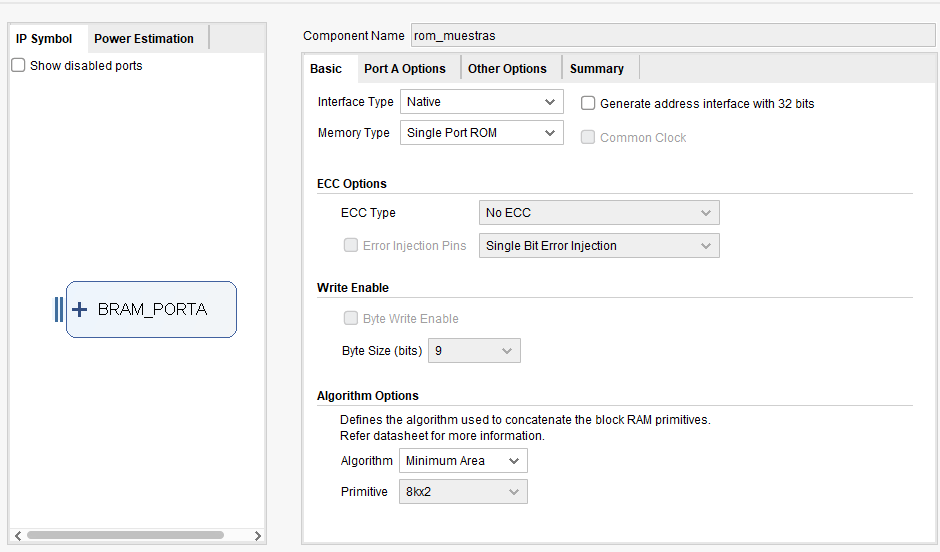
\includegraphics[width=0.6\textwidth]{./Images/img_implementacion_hw/rom_muestras_1.png}
    \caption{Seleccion de la opcion simple block ROM y}
    \label{fig:rom_muestras_1}
\end{figure}
 Es importante desactivar l a opcion de primitive output para que no se añada un registro extra 
 al principio y la simulacion se ejecute en cada tiempo correspondiente. 
\begin{figure}[h!]
    \centering
    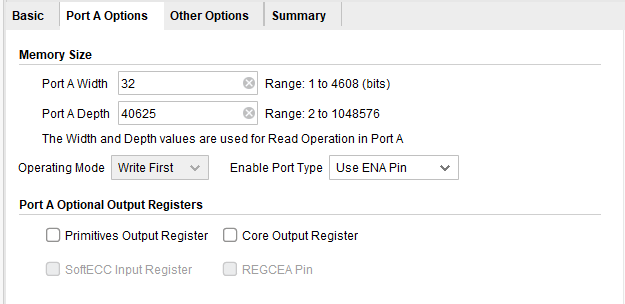
\includegraphics[width=0.6\textwidth]{./Images/img_implementacion_hw/rom_muestras_2.png}
    \caption{Se establecen las filas de la BROM y la longitud de estas}
    \label{fig:rom_muestras_2}
\end{figure}

El modulo de filtrado utiliza 1 ROM y una RAM

\begin{itemize}
\item La ROM se configura igual que la ROM del modulo de input, este tiene 99 filas y de anchura 
tiene 32 bits.
\item La RAM se configura como single port RAM y se mantiene desactivado el valor de primitive output.
 Ahora bien los valores asignados son los siguientes.
 
\begin{figure}[h!]
    \centering
    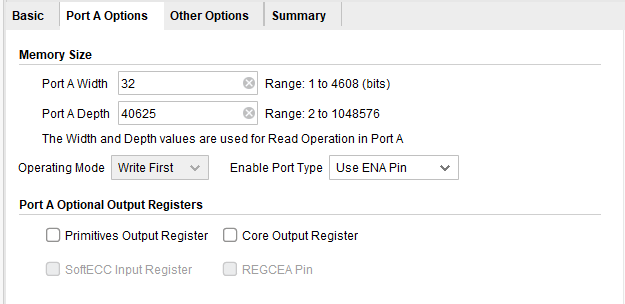
\includegraphics[width=0.6\textwidth]{./Images/img_implementacion_hw/rom_muestras_2.png}
    \caption{Se establecen las filas de lectura y escritura de la RAM y las longitud de dichas filas}
    \label{fig:ram_muestras_1}
\end{figure}

\end{itemize}
